\chapter{The Static Universe: Quantum Cosmology}
\label{chap:wdw}

\section{Everett without Branching}

We have landed in static fully self contained universe which just is. Every possible state of every possible system is already ``compiled" into a single, massive, static lookup table.

This is the Wheeler-DeWitt (WdW) universe. Standard physics often interprets this via the many-worlds (Everettian) view, but with a branching mechanism.
In our informational framework, we refuse to rely on metaphysical branching. There is only a static configuration space $\mathcal{C}$ of $2^n$ bits. Every "Everettian world" is simply a different
configuration in this massive set of information.

The question then is: if everything exists at once, why do we experience a sequential "now"?
As demonstrated earlier, the answer is that we find ourselves along the observer-compatible histories occupying the largest low-complexity equivalence classes.


\section{Quantum Cosmology: Spectral Complexity and the Measure of Observers}

To formalize this, we apply our theory to the scale of the entire cosmos.
In standard quantum cosmology, physicists use a "Wick rotation" to imaginary time to make their math work. 
Rather than relying on Euclidean continuation, we introduce an alternative informational weighting principle based on spectral complexity.


\subsection*{Introduction}

The canonical quantization of general relativity leads to the Wheeler-DeWitt equation \cite{DeWitt1967}:
\begin{equation}
\hat{\mathcal{H}} \Psi[g_{ij}, \phi] = 0,
\end{equation}
where $\Psi$ is the wavefunction of the universe. This equation is timeless. The ``Problem of Time'' arises because all physical predictions must be extracted from a single, static superposition.

In this work, we propose \textit{Spectral Quantum Cosmology} (SQC).
We remain strictly within the static WdW framework and introduce an information-theoretic selection principle based on \textit{Spectral Complexity}.
Rather than weighting geometries via Euclidean action, we weight possible \textit{observer wavefunctions} directly.
Observers with simpler internal descriptions dominate the measure.

\section{Relational Observers in a Timeless Universe}

Following Page and Wootters \cite{page1983clock}, time emerges relationally.
The universal wavefunction $\Psi$ is static and contains entangled subsystems: a clock degree of freedom and the rest of the universe.

An observer corresponds to a wavefunction $\psi_o$ that is entangled with a suitable clock variable $\lambda$ (like the scale factor of the universe).
The experienced flow of time arises from correlations between observer states and relational clock degrees of freedom within the static universal wavefunction.

\subsection*{Intuitive Analogy}

One can think of the universe as divided into two entangled parts:
\begin{itemize}
\item A "clock" subsystem: something that can "tick" (e.g., the position of a particle, the reading on a real clock, the scale factor of the expanding universe, or even a photon's polarization in experiments).

\item The rest of the system: everything else one is interested in (particles, fields, you as an observer, etc.).
\end{itemize}

The total quantum state of the universe is a special entangled superposition. It is completely stationary from the outside — nothing "moves" globally.

However, when one "look at" the state of the clock, the rest of the system appears to change depending on what the clock reads. For example, when the clock reads "10:00," the rest of the universe is in configuration A.
When the clock reads "10:01," the rest of the universe is in configuration B. And so on. 

These correlations can be built into the single static wavefunction.
There is no external time making things evolve.
The appearance of evolution comes purely from asking relational questions: ``Given that my clock shows time t, what is the state of the rest?''

It's like a movie stored on a DVD. The entire film exists all at once on the disc (static). But when you play it and look at the time counter (the clock), scene 5 appears when the counter says 00:05:00, and scene 6 follows at 00:05:01. The story flows *relationally* through the correlation between the counter and the image.

Physicists have actually done tabletop experiments with entangled photons. One photon acts as the "clock," the other as the "system."
An external observer who looks at both photons together sees a static, timeless entangled state.
But an "internal observer" who correlates with the clock photon sees the other photon evolving exactly as quantum mechanics predicts.
Time "emerges" for the insider.

This tames the Problem of Time in a static universed. We don't need an external time parameter. Time is relational.
It fits perfectly with a static configuration space or "block universe" view, and pairs naturally with our low-complexity observers:
the observers who experience smooth, law-like evolution are those strongly correlated with good clock variables in low-complexity ways.

The universe as a whole is timeless and unchanging. But inside it, different parts can be entangled so that *one part acts as a clock for the other*.
What we call "the flow of time" is just reading those built-in correlations — like different frames of a movie that all exist simultaneously, but appear sequential when we watch them with the timecode.


\section{Spectral Complexity as the Measure}

We define the \textit{Spectral Complexity} of an observer wavefunction $\psi_o(\lambda)$ as the minimal information cost of representing it in the frequency domain.
\begin{equation}
\psi_o(\lambda) = \sum_{k=1}^{M} c_k e^{i\omega_k\lambda}
\end{equation}

According to the natural prior weight for any observer:
\begin{equation}
P(\psi_o) \propto 2^{-C_{\text{spec}}(\psi_o)}
\end{equation}

Observers requiring highly oscillatory or spectrally incoherent descriptions are exponentially suppressed.
Conversely, observers who experience smooth, law-like evolution dominate the measure.
This replaces the "imaginary time" trick of standard physics with a native algorithmic measure.




\section{Testing the Idea in a Simple Simulation}

We implemented a minimal simulation (2 spatial and 1 time dimension) to see if our "Minimal Complexity" path matched the "Least Action" path of traditional physics.

\begin{figure}[h]
\centering
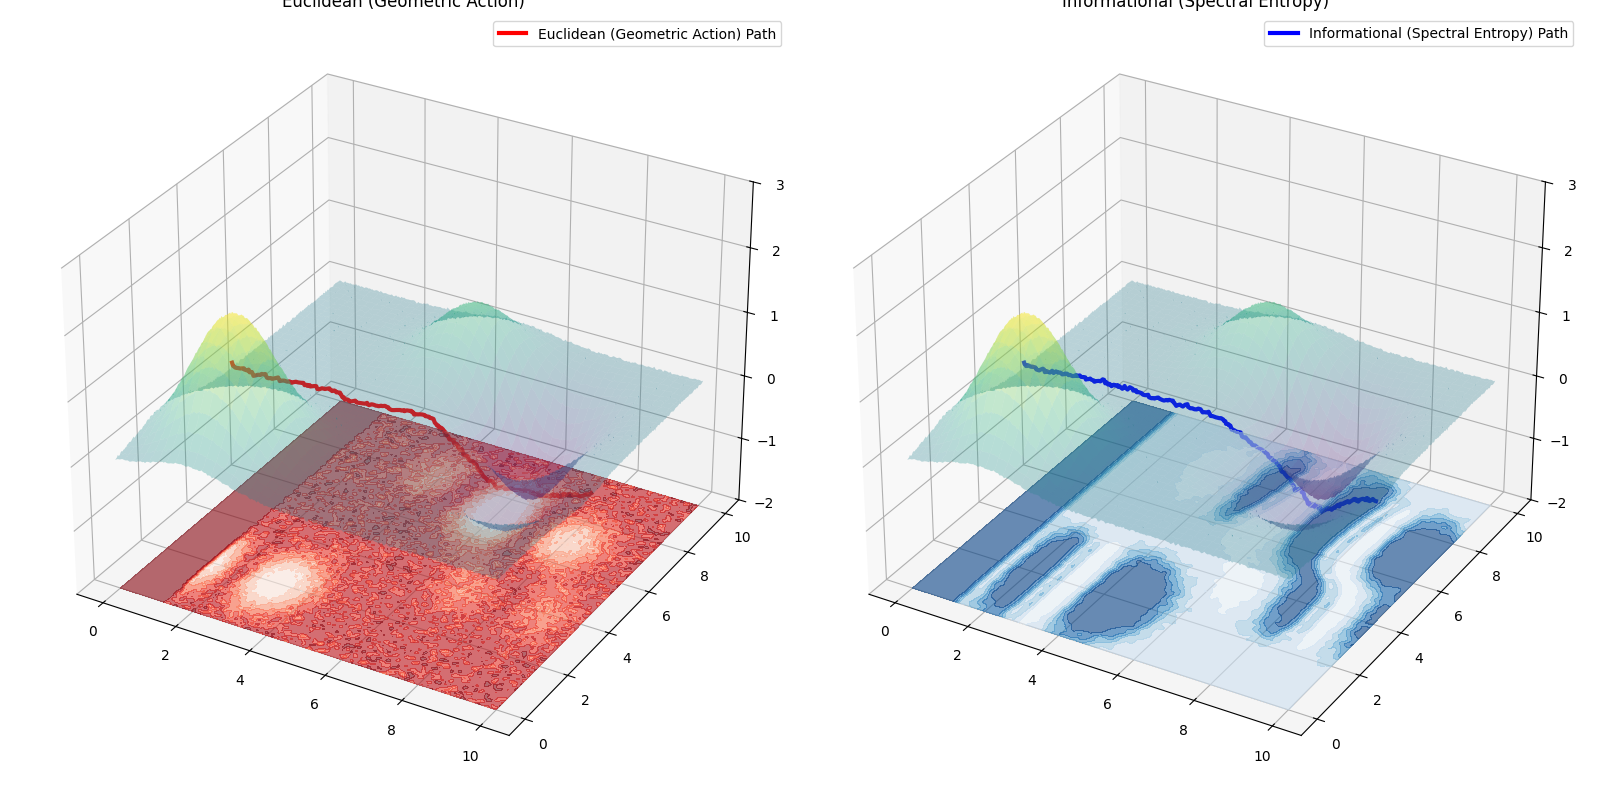
\includegraphics[width=0.8\textwidth]{figures/wdwfields.png}
\caption{Side-by-side comparison: The classical field (Euclidean Action) vs.
  The Informational field (Induced Measure). Preliminary numerical results indicate rough agreement between minimal spectral complexity trajectories and classical least-action solutions.}
\end{figure}


\begin{figure}[h]
\centering
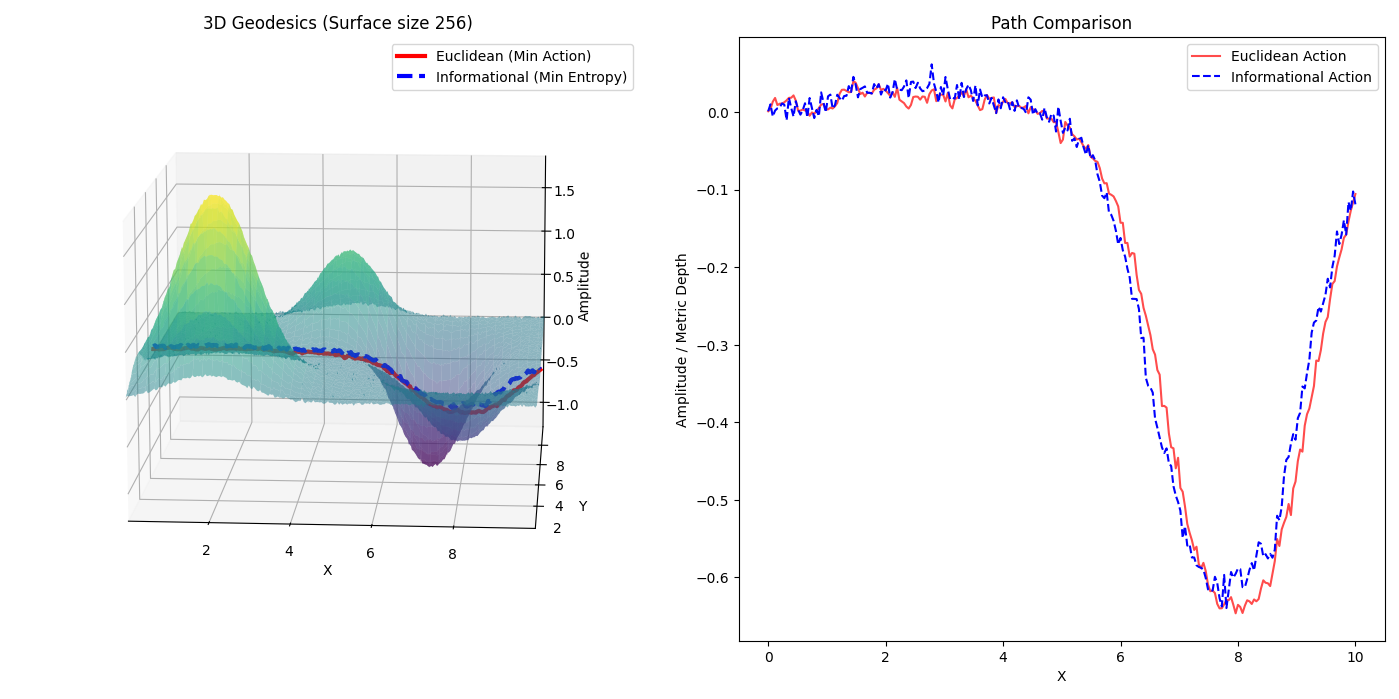
\includegraphics[width=0.8\textwidth]{figures/wdwpaths.png}
\caption{Side-by-side comparison: The classical path (Euclidean Action) vs.
  The Informational path (Induced Measure). Preliminary numerical results indicate strong qualitative agreement between minimal spectral complexity trajectories and classical least-action solutions.}
\end{figure}


The results were promising. 
The path that is "simplest to describe" spectrally matches approximately the path that Einstein’s equations predict.
The apparent fuzziness of microscopic physics may reflect limitations inherent in finite observer-side spectral representation.

\section{Conclusion}

When applied to cosmology, the framework naturally converges toward an effective Wheeler--DeWitt description:
a timeless, self-contained universe in which dynamics emerge relationally through observer-conditioned correlations.


\section{Future Work}

The simulations were 2D toy-models with predefined metric without backreaction.
Implement a true closed FLRW minisuperspace simulation.
